\documentclass[../main.tex]{subfiles}
%!TEX root = ./analysisDragAnalysis.tex
\graphicspath {{../}}

\begin{document}
\subsection{Drag Analysis}

An analysis from a report called \textit{Technical Manual of Airship Aerodynamics} \cite{airshipAerodynamics} was used to determine the effect of drag on the airship. The following formula was used to compute the total drag force:

\begin{equation*}
		D = C_D\rho (vol)^{2/3}v^{1.86}
\end{equation*}

Where $D$ is the drag in $lbf$, $ \rho $ is the density of air $[slugs/ft^3]$, $vol$ is the volume of the airship envelope $[ft^3]$, $v$ is the velocity of the airship $[ft/s]$, and $C_D$ is the Prandtl Shape Coefficient.\\

The formula is converted into metric units for simplicity, using a multiplication factor:

\begin{equation} \label{eqnDrag}
D[N] = 0.847103*(C_D)*(\rho[kg/m^3])*(vol [m^3])^{2/3}*(v [m/s])^{1.86}
\end{equation}

For this airship, $C_D$ is estimated using Table \ref{tbl:airshipTableCont} below.\\

\begin{table}[H]
	\centering
	\caption{Airship Model Characteristics and Data \cite{airshipAerodynamics} Continued}
	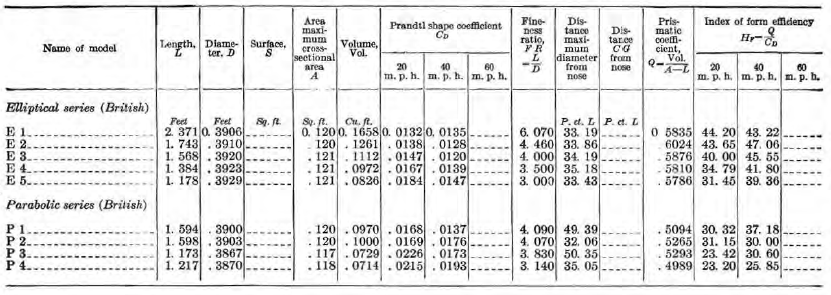
\includegraphics[width=\linewidth]{img/drag/airships2.PNG}
	\label{tbl:airshipTableCont}
\end{table}


The aircraft dimensions shown in Table \ref{tbl:airshipTableCont} are results of testing  in a wind tunnel, used to determine drag effects on real airships. They are therefore scaled down models. The goal is to select a model that has comparable dimensions to the airship to be constructed for this project.\\

It can be deduced from the table that the Prandtl Shape coefficient encompasses both skin and form drag. When the fineness ratio is higher, skin friction drag will have a larger effect than form drag, so when the airspeed is increased (from 20mph to 60mph), $C_D$ will decrease. The opposite is true with small fineness ratios, where the form drag plays a larger role, therefore the $C_D$ increases as airspeed is increased. \\

As a example, assuming the blimp designed has a fineness ratio of 3.5, the comparable blimp would be the Elliptical series E 4. To be conservative, the highest $C_D$ from the E 4 is $C_D = 0.0167$. The calculation is shown below, for a windspeed of $20m/s$:

\begin{equation*} \label{exDrag}
D = C_D\rho (vol)^{2/3}v^{1.86}=0.0167*(0.00237 slugs/ft^3)*(122.644 ft^3)^{2/3}(65.616 ft/s) ^{1.86} = 2.342 lbf = 10.417735N 
\end{equation*}

Based on Table \ref{tbl:contributionsTable}, the envelope contributes 45\% to the drag. Therefore the total drag will be estimated as $D_{total}=D/0.45$. Based on this, the total drag in found in Equation \ref{exDrag} is now $23.15N$.

\begin{table}[H]
	\centering
	\caption{Drag Contribution for Various Airship Components \cite{airshipAerodynamics}}
	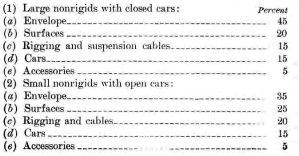
\includegraphics[width=.5\linewidth]{img/drag/contributions.PNG}
	\label{tbl:contributionsTable}
\end{table}

These estimates are meant to be extremely conservative, due to the fact that the construction of the blimp will not be perfect, and any modelling situation will not be able to capture all of the imperfections in the build.\\

The value of $C_D$ will change based on the fineness ratio. In the GUI of the MATLAB program, the user will input the dimensions of the airship, and the program will calculate $C_D$ based on the fineness ratio ($fr$). The GUI will only allow the user to input dimensions which result in fineness ratios of between 3.0 and 4.0. This is due to the fact that these fineness ratios most accurately reflect the shape of the pre-existing keel. The relationship is found by curve-fitting the data in Table \ref{tbl:finenessCoefficient}, which were obtained from values in Table \ref{tbl:airshipTableCont}.

\begin{table}[H]
	\caption{Fineness Ratios and Corresponding $C_D$}
	\label{tbl:finenessCoefficient}
\begin{center}
	\begin{tabular}{|c|c|}
	\hline 
	\textbf{Fineness Ratio $fr$} & \textbf{$C_D$} \\ 
	\hline 
	3.000 & 0.0184 \\ 
	\hline 
	3.500 & 0.0167 \\ 
	\hline 
	4.000 & 0.0147 \\ 
	\hline
	4.460 & 0.0138 \\ 
	\hline 
	6.070 & 0.0132 \\ 
	\hline  
\end{tabular} 
\end{center}
\end{table}

The resulting equation for drag coefficient is found as:

\begin{equation} \label{eqnCD}
	C_D(fr)= 0.00092642*fr^2 -0.010134*fr + 0.040569
\end{equation}

Equations \ref{eqnDrag} and \ref{eqnCD} are used in conjunction to determine the drag force acting on the blimp.

\end{document}